\documentclass{standalone}

\usepackage{tikz}
\usetikzlibrary{shapes.misc}

\begin{document}

% \resizebox{10cm}{!}{
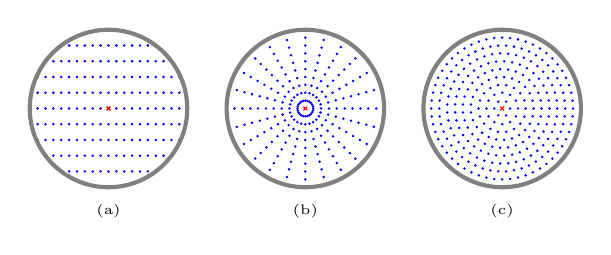
\begin{tikzpicture}[
    dot/.style={circle,draw=none,fill=blue,inner sep=0pt},
    origin/.style={cross out,draw=red,inner sep=0pt,minimum size=1pt},
    line/.style={black!50,line width=1.5pt}
]
    % Homogeneous anisotropic distribution
    \pgfmathsetmacro{\xoff}{1}
    \pgfmathsetmacro{\yoff}{1}

    \foreach \x in {-1.0, -0.9, ..., 1.0} {
        \foreach \y in {-1.0, -0.8, ..., 1.0} {
            \pgfmathparse{\x*\x + \y*\y <= 1 && \x*\x + \y*\y > 0}
            \ifnum\pgfmathresult=1
                \pgfmathsetmacro{\newx}{\x + \xoff}
                \pgfmathsetmacro{\newy}{\y + \yoff}
                \node[dot] at (\newx, \newy) {};
            \fi
        }
    }

    \node[origin] at (\xoff, \yoff) {};
    \draw[line] (\xoff, \yoff) circle (1) node[yshift=-1.3cm,color=black]{\tiny (a)};

    %%%%%%%%%%%%%%%%%%%%%%%%%%%%%%%%%%%%%%%%%%%%%%%%%%%%%%%%%%%%%%%%%%%%%%%%%%%%%%%%%%%%

    % Inhomogeneous isotropic distribution
    \pgfmathsetmacro{\xoff}{3.5}

    \foreach \r in {0.1, 0.2, ..., 1.0} {
        \foreach \t in {0, 15, ..., 359} {
            % \pgfmathsetmacro{\newr}{\r + 0.05 * \r * rand}
            % \pgfmathsetmacro{\newt}{\t + rand}
            \pgfmathsetmacro{\newr}{\r}
            \pgfmathsetmacro{\newt}{\t}
            \pgfmathsetmacro{\x}{\newr * cos(\newt) + \xoff}
            \pgfmathsetmacro{\y}{\newr * sin(\newt) + \yoff}
            \node[dot] at (\x, \y) {};
        }
    }

    \node[origin] at (\xoff, \yoff) {};
    \draw[line] (\xoff, \yoff) circle (1) node[yshift=-1.3cm,color=black]{\tiny (b)};

    %%%%%%%%%%%%%%%%%%%%%%%%%%%%%%%%%%%%%%%%%%%%%%%%%%%%%%%%%%%%%%%%%%%%%%%%%%%%%%%%%%%%

    % Homogeneous isotropic distribution
    \pgfmathsetmacro{\xoff}{6}

    \foreach \r in {0.1, 0.2, ..., 1.0} {
        \pgfmathsetmacro{\dtheta}{360 / int(2 * pi * \r / 0.1)}
        \foreach \t in {0, \dtheta, ..., 359} {
            % \pgfmathsetmacro{\newr}{\r + 0.05 * \r * rand}
            % \pgfmathsetmacro{\newt}{\t + rand}
            \pgfmathsetmacro{\newr}{\r}
            \pgfmathsetmacro{\newt}{\t}
            \pgfmathsetmacro{\x}{\newr * cos(\newt) + \xoff}
            \pgfmathsetmacro{\y}{\newr * sin(\newt) + \yoff}
            \node[dot] at (\x, \y) {};
        }
    }

    \node[origin] at (\xoff, \yoff) {};
    \draw[line] (\xoff, \yoff) circle (1) node[yshift=-1.3cm,color=black]{\tiny (c)};
\end{tikzpicture}
% }
\end{document}
